%sparse_matrize

Sparse Matrize\\
Sparsematrizen, oder dünnbesetzte Matrizen,  bezeichnet man als eine Matrizen, bei der so viele Einträge aus Nullen bestehen. Im Fig 1 wird ein einfaches Beispiel gezeigt.
Da Sparsematrizen mit Vollmatrizen genau umgekehrt ist, hat man dafür auch eine andere Speicherweise. Unter dem Zusammenhang zwischen Fig.\ref{orignal_sparse}., Fig.\ref{numerische_sparse1}. und Fig.\ref{numerische_sparse2}. versteht man, dass bei der Sparsematrizen wird nun nur die Nonzero-Elementeund und die zugehörigen Stelleinformationen(Zeilen und Spalte) gespeichert. Vektor \textquotedblleft pr \textquotedblright enthält alle Nonzero-Elemente. Die Vektoren \textquotedblleft ir\textquotedblright und \textquotedblleft jc\textquotedblright enthalten die Zeileninformation und die Spalteinformation. Im Fig.\ref{numerische_sparse2}. bezeichnet man, wie die Informationen gepackt werden. Die Werte von \textquotedblleft jc[i]\textquotedblright und \textquotedblleft jc[i+1]-1\textquotedblright zeigen den Indexe, deren die zur Spalte \textquotedblleft i\textquotedblright  gehörteten Nonzero-Elemente und Zeileinformation aufweisen.

%\begin{figure}[htbp]
%	\includegraphics[width=1in]{.//pic//orignal_sparse}
%	\caption{Original-Matrize}
%	\includegraphics[width=1in]{.//pic//numerische_sparse1}
%	\caption{Sparsame Struktur}
%	\includegraphics[width=1in]{.//pic//numerische_sparse2}
%	\caption{compressed column structure"}
%\end{figure}

% \begin{figure}[htbp]
	% \begin{center}
		% \begin{minipage}[t]{0.4\linewidth}
			% \centering
			% \includegraphics[width=\linewidth]{../xby/pic/orignal_sparse}
			% \caption{Original-Matrize}
			% \label{orignal_sparse}
		% \end{minipage}
		% \qquad
		% \begin{minipage}[t]{0.4\linewidth}
			% \centering
			% \includegraphics[width=\linewidth]{../xby/pic/numerische_sparse1}
			% \caption{Sparsame Struktur}
			% \label{numerische_sparse1}
		% \end{minipage}
		% \qquad
		% \begin{minipage}[t]{0.4\linewidth}
			% \centering
			% \includegraphics[width=\linewidth]{../xby/pic/numerische_sparse2}
			% \caption{"compressed column structure"}
			% \label{numerische_sparse2}
		% \end{minipage}
	% \end{center}
% \end{figure}

\begin{figure}[htbp]
  \centering
     \subfloat[][Original-Matrize]{\label{fig:orignal_sparse}\includegraphics[width=2.5cm]{../xby/pic/orignal_sparse}}
	 \hspace{0.5cm}
	\subfloat[][Sparsame Struktur]{\label{fig:numerische_sparse1}\includegraphics[width=2.5cm]{../xby/pic/numerische_sparse1}}
	\hspace{0.5cm}
	\subfloat[]["compressed column structure"]{\label{fig:numerische_sparse2}\includegraphics[width=2.5cm]{../xby/pic/numerische_sparse2}}	 
  \caption{Sparse Matrix}
  \label{fig:animals}
\end{figure}